\documentclass[12pt]{article} 

\usepackage{geometry} 
\geometry{a4paper} 
\usepackage{graphicx} 
\usepackage{float} 
\usepackage{wrapfig} 
\linespread{1.2}
\graphicspath{{Pictures/}} 
\usepackage[utf8]{inputenc}
\usepackage[T1]{fontenc}
\usepackage[portuguese]{babel}

\begin{document}

%----------------------------------------------------------------------------------------
%	TITLE PAGE
%----------------------------------------------------------------------------------------

\begin{titlepage}

\newcommand{\HRule}{\rule{\linewidth}{0.5mm}} 
\center
\begin{figure}[ht!]
	\centering
	
\includegraphics[scale=3]{DI.png}
\end{figure}

\textsc{\large Sistemas Operativos}\\[0.5cm] 
\HRule \\[0.4cm]
{ \huge \bfseries Stream Processing}\\[0.4cm] 
\HRule \\[1.5cm]


\begin{center} \large
\emph{Grupo 19:}\\
José Martins - a78821\\
Madalena Castro - a71417\\
Miguel Quaresma - a77049\\
\end{center}

\begin{minipage}{0.4\textwidth}
\end{minipage}\\[4cm]

{\large \today}\\[3cm] 
\vfill
\end{titlepage}

%----------------------------------------------------------------------------------------
%	TABLE OF CONTENTS
%----------------------------------------------------------------------------------------

\tableofcontents 

\newpage

%----------------------------------------------------------------------------------------
%	INTRODUÇÃO
%----------------------------------------------------------------------------------------

\section{Introdução}
\texit{Stream Processing} é uma arquitetura computacional que tem como intuito facilitar o uso de paralelismo no processamento de dados ao abstrair o utilizador da gestão dos recursos disponíveis (i.e: comunicação entre nodos, uso de recursos,etc). Os dados são recebidos sob a forma de streams e operações que são aplicadas a cada elemento da stream. 

A linguagem de programação C disponibiliza um conjunto de chamadas ao sistema que permitem a exploração de paralelismo simples, sendo o intuito deste trabalho recorrer a estas mesmas chamadas para implementar um sistema similar ao referido.


\newpage

%----------------------------------------------------------------------------------------
%	DESENVOLVIMENTO
%----------------------------------------------------------------------------------------

\section{Desenvolvimento} 

\subsection{Estrutura}

\subsection{Controlador}
O controlador é a entidade responsável por processar input e gerir a rede de processamento, nomeadamente através da criação/remoção de nodos e gestão das ligações entre os mesmos.
A gestão dos nodos recorre a três arrays para manter informação relativa às ligações entre os nodos, ao pid(process id) dos mesmos e aos descriptores dos nnamed pipes que servem de input para os nodos.
A leitura do input é feita linha a linha através de um named pipe com o nome \textit{input}, de seguida o input é classificado como instruções ou dados através da presença(ou ausência) do caracter ':'.
Os comandos disponíveis são os seguintes:
\begin{itemize}
\item \texttt{node}: criação de um novo nodo, executado pela função \texttt{newNode}
\item \texttt{connect}: ligação de nodos entre si, executado pela função \texttt{connect}
\item \texttt{inject}: usado para providenciar input adicional aos nodos por meio da execução de um comando, executado pela função \texttt{inject}
\item \texttt{disconnect}: usado para remover ligações entre nodos, executado pela função \texttt{disconnect}
\item \texttt{remove}: remoção de um nodo, executado pela função \texttt{removeNode}
\end{itemize}
Determinados comandos exigem ações por parte dos nodos e, por forma a que estes sejam diferentes dos dados enviados para os mesmos(nodos) é usado como prefixo o caracter ';' seguido de um caracter que identifique o comando a executar ('c' para \textit{connect} e 'd' para \textit{disconnect}).

\begin{figure}[ht!]
     \centering
         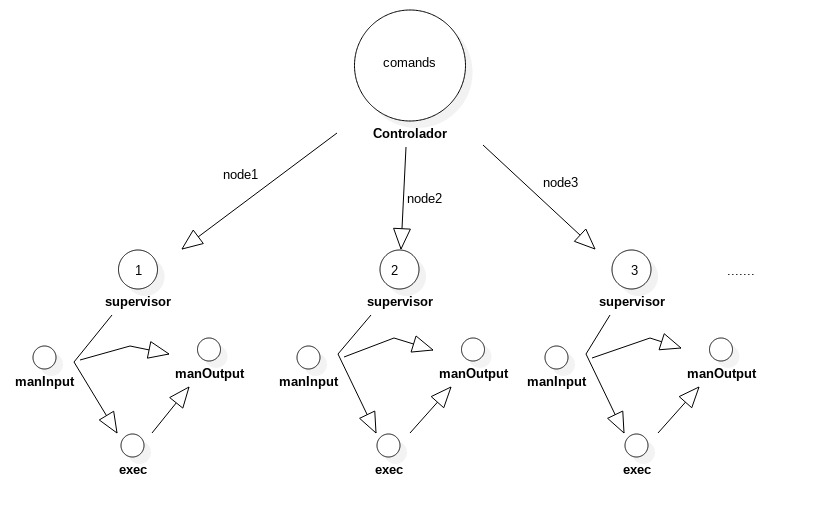
\includegraphics[width=120mm]{graph.jpg}
     \caption{}
\end{figure}


\subsubsection{Makefile}
A makefile compila os ficheiros responsáveis pelas componentes (\texttt{const},  \texttt{filter}, \texttt{window}, \texttt{spawn}) e os ficheiros responsáveis pelo controlador (\texttt{controler}, \texttt{commands}, \texttt{supervisor}), utilizando as flags \texttt{g} e \texttt{Wall}. Também é responsável pela eliminação de todos os ficheiros objeto criados durante a compilação.

\subsubsection{iStormAPI.h}
O ficheiro iStormAPI.


\subsection{Componentes} 
\begin{description} 
\item[Const] \hfill \\
O componente \textit{const} reproduz as linhas recebidas acrescentando uma nova coluna sempre com o mesmo valor. Para isso, lemos caractér a caractér recebido pelo \textit{stdin} e após verificar que estamos no término de uma linha ('\textbackslash n'), adicionamos uma nova coluna com o valor dado como argumento. Posteriormente, concluímos a linha com '\textbackslash n', e reproduzimo-la no \textit{stdout}, realizando esta operação para todas as linhas recebidas. 

\item[Filter] \hfill \\
O componente \textit{filter} reproduz as linhas que satisfazem uma condição passada como argumento. Esta condição é composta por um operador de comparação e dois valores que correspondem a colunas das linhas a ser processadas. Inicialmente começamos por dividir a linha recebida pelo \textit{stdin} consoante o \textit{token} ':',caso estejamos numa linha presente na condição guardamos o valor numa variavel local, para posteriormente verificarmos a condição recebida, caso verdadeira a linha será reproduzida no \textit{stdout}, caso falso será desprezada.

\item[Window] \hfill \\
O componente \textit{window} reproduz todas as linhas acrescentando-lhe uma nova coluna com o resultado de uma operação calculada sobre valores da coluna indicada nas linhas anteriores. Inicialmente começamos por verificar os argumentos recebidos, guardando a coluna, a operação e quais as linhas anteriores a serem calculadas. De seguida, começámos a leitura das linhas recebidas pelo \textit{stdin} e à medida que uma linha termina é reproduzido no \textit{stdout} a linha com a coluna que representa o cálculo da operação, previamente calculada consoante o tipo de operação, ou seja, inicialmente, como não há linhas anteriores a nova coluna será zero, mas consoante o avanço das linhas será recalculado o valor da nova coluna e guardado numa variável que será posteriormente utilizada para criar a nova coluna. Consoante o tipo de operação enviada como argumento, criámos diferentes funções.

\item[Spawn] \hfill \\
    O componente \textit{spawn} reproduz todas as linhas, executando o comando indicado uma vez para cada uma delas, e acrescentando uma nova coluna com o respectivo \textit{exit status}. É permitido o uso de \textit{'\$n'} no qual é indicado o número de uma coluna das linhas, de modo a que ao executar o comando, nos seus argumentos na posição do \textit{'\$n'} esteja o conteúdo presente na coluna n de cada linha. Para tal, vamos lendo a linha, caracter a caracter, e quando encontramos a/s coluna/s especificada/s guardamos o conteudo numa variavel local. Quando chegamos ao '\textbackslash n' executamos o argumento num filho, porém tendo o cuidado de substituir as partes com '\$n' pelo correto conteúdo.  

\end{description} 

\subsection{Controlador}
O controlador é a entidade responsável pela gestão da stream de dados e das operações realizadas
O controlador é um programa que permite definir uma rede de processamento de \textit{streams}, com cada nó a executar um dos componentes de transformação previamente feitos, recebendo comandos, um por linha. 

\subsubsection{commands}
O ficheiro \texttt{commands.c} contém as funções necessárias para realizar os comandos que o controlador deve aceitar, sendo esses os seguintes:

\begin{description} 
\item[newNode] \hfill \\
    Função que realiza o comando \texttt{node <id> <cmd> <args...>}, definindo um nó de rede de processamento, com o indentificador  \texttt{id}, que executará o componente \texttt{cmd} com a lista de argumentos \texttt{[args]}. Para tal,começamos por criar um pipe com nome com o nome "nodeid", sendo que na posição do id estará o número do nodo, este pipe com nome como já indicado irá servir para o nodo receber input bem como comandos do controlador. De seguida tratamos de "criar" o nodo realmente ao criar um filho e colocar nele em execução o binario \texit{supervisor}. Por fim, abrimos o pipe com nome, guardando o \texit{file descriptor} do mesmo num array, sendo que guardamos também o \texit{process ID} necessário para posteriores ações sobre o supervisor.

\item[connect] \hfill \\
Função que realiza o comando \texttt{connect <id> <ids...>}, que permite definir ligações entre nós, ou seja, especifica que a saída do componente a correr no nó \texttt{id} deverá ser enviada para cada um dos nós da lista \texttt{[ids]}. 
\\Esta função recebe como argumentos um \textit{array} com o \texttt{id} e os \texttt{[ids]} a conectar, um \textit{array} de inteiros com os pipes e a lista ligada com os estados dos nós.
\\..... 

\item[inject] \hfill \\
Função que realiza o comando \texttt{inject <id> <cmd> <args...>}, que permite injetar na entrada do nó \texttt{id} a saída produzida pelo comando cmd executado com a lista de argumentos \texttt{[args]}. 
\\Esta função recebe como argumentos um \textit{array} de argumentos dada pelo \textit{stdin} e  um \textit{array} de inteiros com os pipes.
\\.......

\item[disconnect] \hfill \\
Função que realiza o comando \texttt{disconnect <id1> <id2>}, que permite desfazer a ligação entre o nó \texttt{id1} e o nó \texttt{id2}. 
\\Esta função recebe como argumentos um \textit{array} de argumentos dada pelo \textit{stdin}, um \textit{array} de inteiros com os pipes, e a lista ligada com os estados dos nós.
\\......

\item[removeNode] \hfill \\
Função que realiza o comando \texttt{remove <id>}, que permite a remoção de um nó na rede. 
\\Esta função recebe como argumento um \textit{array} de argumentos dada pelo \textit{stdin}, a lista ligada com os estados dos nós, um \textit{array} de inteiros com os pipes, um inteiro correspondente ao número de nós ativos, e um inteiro correspondente ao número de nós.
\\...... 
\end{description}

\subsubsection{supervisor}


\subsection{Funcionalidades básicas}
\begin{description} 

\item[Permanência de uma rede] \hfill \\
Os nós de uma rede, depois de criados, continuam a existir até serem explicitamente removidos. Esta deve ficar recetiva a processar \textit{streams} de eventos que parem e recomecem mais tarde.

\item[Concorrência nas escritas no mesmo nó] \hfill \\
Ao especificar uma rede, vários nós podem ser ligados a um mesmo nó, ou várias instâncias do comando \texttt{inject}, com outras ainda a decorrer. Como tal, o sistema deve garantir que cada evento chega corretamente ao destino, não corrompido, havendo apenas intercalamento de eventos de diferentes origens.

\item[Nós sem saída definida] \hfill \\
Os nós cuja saída não esteja ligada a nenhum outro devem ter a sua saída descartada.

\item[Especificação incremental na rede] \hfill \\
O servidor vai recebenco comandos, devendo atuar perante cada um, atualizando a rede, independentemente de comandos futuros.

\end{description}

\subsection{Funcionalidades adicionais}

\begin{description} 
\item[Casos de teste] \hfill \\
rrrrr

\item[Alteração de componentes] \hfill \\
aaaa

\item[Remoção de nós] \hfill \\
ggg


\end{description}

\newpage
%----------------------------------------------------------------------------------------
%	CONCLUSÃO
%----------------------------------------------------------------------------------------

\section{Conclusão} 

ESCREVER CONCLUSAO! 


%----------------------------------------------------------------------------------------

\end{document}
